\documentclass[11pt,]{article}
\usepackage{lmodern}
\usepackage{amssymb,amsmath}
\usepackage{ifxetex,ifluatex}
\usepackage{fixltx2e} % provides \textsubscript
\ifnum 0\ifxetex 1\fi\ifluatex 1\fi=0 % if pdftex
  \usepackage[T1]{fontenc}
  \usepackage[utf8]{inputenc}
\else % if luatex or xelatex
  \ifxetex
    \usepackage{mathspec}
    \usepackage{xltxtra,xunicode}
  \else
    \usepackage{fontspec}
  \fi
  \defaultfontfeatures{Mapping=tex-text,Scale=MatchLowercase}
  \newcommand{\euro}{€}
\fi
% use upquote if available, for straight quotes in verbatim environments
\IfFileExists{upquote.sty}{\usepackage{upquote}}{}
% use microtype if available
\IfFileExists{microtype.sty}{%
\usepackage{microtype}
\UseMicrotypeSet[protrusion]{basicmath} % disable protrusion for tt fonts
}{}
\usepackage[margin=1in]{geometry}
\usepackage{natbib}
\bibliographystyle{plainnat}
\usepackage{longtable,booktabs}
\usepackage{graphicx}
\makeatletter
\def\maxwidth{\ifdim\Gin@nat@width>\linewidth\linewidth\else\Gin@nat@width\fi}
\def\maxheight{\ifdim\Gin@nat@height>\textheight\textheight\else\Gin@nat@height\fi}
\makeatother
% Scale images if necessary, so that they will not overflow the page
% margins by default, and it is still possible to overwrite the defaults
% using explicit options in \includegraphics[width, height, ...]{}
\setkeys{Gin}{width=\maxwidth,height=\maxheight,keepaspectratio}
\ifxetex
  \usepackage[setpagesize=false, % page size defined by xetex
              unicode=false, % unicode breaks when used with xetex
              xetex]{hyperref}
\else
  \usepackage[unicode=true]{hyperref}
\fi
\hypersetup{breaklinks=true,
            bookmarks=true,
            pdfauthor={Michael C Sachs and Lisa M McShane},
            pdftitle={Issues in developing multivariable molecular signatures for guiding clinical care decisions},
            colorlinks=true,
            citecolor=blue,
            urlcolor=blue,
            linkcolor=magenta,
            pdfborder={0 0 0}}
\urlstyle{same}  % don't use monospace font for urls
\setlength{\parindent}{0pt}
\setlength{\parskip}{6pt plus 2pt minus 1pt}
\setlength{\emergencystretch}{3em}  % prevent overfull lines
\setcounter{secnumdepth}{0}

%%% Use protect on footnotes to avoid problems with footnotes in titles
\let\rmarkdownfootnote\footnote%
\def\footnote{\protect\rmarkdownfootnote}

%%% Change title format to be more compact
\usepackage{titling}

% Create subtitle command for use in maketitle
\newcommand{\subtitle}[1]{
  \posttitle{
    \begin{center}\large#1\end{center}
    }
}

\setlength{\droptitle}{-2em}
  \title{Issues in developing multivariable molecular signatures for guiding
clinical care decisions}
  \pretitle{\vspace{\droptitle}\centering\huge}
  \posttitle{\par}
  \author{Michael C Sachs and Lisa M McShane}
  \preauthor{\centering\large\emph}
  \postauthor{\par}
  \predate{\centering\large\emph}
  \postdate{\par}
  \date{May 18, 2016}

\usepackage{setspace}
\doublespacing
\usepackage{lineno}
\linenumbers


\begin{document}

\maketitle


\section{Abstract}\label{abstract}

Omics technologies that generate a large amount of molecular data
characterizing patient biospecimens have the potential to provide
information about patients' disease characteristics above and beyond
standard clinical and pathological features. By combining the
information from a large number of molecular features into a
multivariable model or decision algorithm, called a biomarker signature,
there is the opportunity to identify distinct subgroups of patients for
whom treatment decisions can be personalized. A biomarker signature can
guide decisions to treat or not to treat and help identify the patients
who are most likely to have a more favororable outcome or benefit from a
particular therapy. The key challenge is to combine features from a high
dimensional molecular assay to derive a signature with good clinical
performance and appropriately characterize its performance. The
inappropriate practice of using overlapping data to both build a
signature and evaluate its performance can lead to severe over-optimism
bias in performance estimates. We summarize the key statistical issues
and methods for developing and validating biomarker signatures, using
examples from the literature for illustration.

\section{Introduction}\label{introduction}

Omics technologies that generate a large amount of molecular data
characterizing patient biospecimens have the potential to provide
information about the patients' disease characteristics above and beyond
standard clinical and pathological features. By combining the
information from a large number of molecular features into a
multivariable model, hereafter referred to as a \emph{biomarker
signature}, there is the opportunity to identify distinct subgroups of
patients for whom clinical management decisions can be personalized. In
early-stage disease, for example, a highly prognostic signature might
identify a subpopulation of good risk patients that has such a high
probability of long survival or disease-free survival that they do not
require additional treatment beyond some standard base therapy.
Therefore these good risk patients can be spared the risks and
side-effects associated with additional therapy. In the context of a
specific therapy that targets a particular molecular pathway, a
signature may identify a subpopulation of patients that does or does not
benefit from that therapy, thereby guiding the decision of whether or
not to administer the therapy.

The key challenge we address in this paper is how to combine feature
mneasurements generated by a high dimensional multiplex molecular assay
to derive a signature that is fit for a specified clinical and
additionally provide valid estimates of its performance characteristics.
A signature that has clinical value must have statistical performance
(as quantified by one or more metrics) that is fit for the clinical
context, and it must provide information that can be acted upon
clinically to provide some benefit to a patient. For example, a
biomarker signature that is well calibrated may accurately predict a
clinical outcome, but that does not neccessarily imply that the
prediction provides clinically useful information; the signature may
divide patients into subgroups with different prognosis, but if there
are no therapies available to improve the outcome of either subgroup,
then the signature may have little clinical value. While the focus here
is statistical estimation of a numerical performance metric, it should
be kept in mind that clinical usefulness may depend on a variety of
additional factors.

\subsection{Terminology and Notation}\label{terminology-and-notation}

A \textbf{biomarker signature} is a transformation of multiple
individual feature measurements, typically molecular characteristics
measured on a multiplex assay, to a one-dimensional space. Specifically,
let \(X\) denote the set of \(p\) feature measurements under
consideration. The signature is an unknown function
\(f(X): \mathbb{R}^p \mapsto \mathbb{R}^1\). The signature result may be
continuous, take multiple discrete values, or be dichotomous. In
principle, the signature could also depend on other clinical or
pathological variables in addition to the molecular measurements, but to
simplify the discussion we will focus on signatures that depend on
molecular feature data only. Let \(S\) denote the development dataset
which includes, for each of \(n\) represented individuals, a feature
vector \(X\), an outcome \(Y\), and a treatment \(Z\). \(S\) is a sample
of size \(n\) from distribution \(\mathcal{P}\) with domain
\(\mathcal{S}\). Let \(\mathcal{F}\) be a mapping from \(\mathcal{S}\)
to the space of continuous functions, \(\mathcal{D}\), with domain
\(\mathbb{R}^p\) and range \(\mathbb{R}\). Thus
\(\mathcal{F}: \mathcal{S} \mapsto \mathcal{D}\) denotes the process or
algorithm through which a particular \(f\) is estimated. We do not place
any other restrictions on \(\mathcal{F}\), it could be a clustering
approach, a regression approach, a combination of both, or something
else entirely. We will use \(\mathcal{F}\) to denote the manner in which
\(f\) is estimated and will write \(f \in \mathcal{F}\) to denote that
\(f\) is estimated with the class of methods \(\mathcal{F}\).

Let \(\phi: \mathcal{D} \times \mathcal{S} \mapsto \mathbb{R}\) denote
the statistic that quantifies the performance of the function \(f\),
such as predictive accuracy, mean squared error, or area under the
receiver operating characteristic (ROC) curve (AUC). This could also be
a measure of association, such as an odds ratio, hazard ratio, or
log-rank statistic. This is a function of both \(f\) and \(S\). We are
interested in estimating \(E_\mathcal{P}[\phi_{f^*}(S)]\), which is the
expected error under the data generation mechanism (distribution
\(\mathcal{P}\)), for a particular \(f^* \in \mathcal{F}\). This allows
us to understand how the signature will perform on future observations
generated from \(\mathcal{P}\). We may also be interested in estimating
\(E_\mathcal{P}[\phi_f(S)]\) \textbf{for all} \(f \in \mathcal{F}\),
which is the generalization performance for \(f\) generated using
mechanism \(\mathcal{F}\). This doesn't guide outside researchers as to
which specific \(f\) to use, yet it is useful for development because it
tells us how much signal is in the data. As shorthand we will write this
as \(E_\mathcal{P}[\phi_\mathcal{F}(S)]\).

\subsection{Overview of biomarker signature
development}\label{overview-of-biomarker-signature-development}

The inherent statistical challenge is how to both develop a signature
\(f \in \mathcal{F}\) and obtain a valid assessment of its performance.
Additionally, one should provide a specification of \(f\) for others to
use. Typically, a specific \(f\) is estimated using \(\mathcal{F}\)
based on some training data. The class of methods \(\mathcal{F}\) can
comprise a variety of different computational approaches. In recent
years there has been an explosion in the literature of computational
approaches to classification and prediction, and we do not intend to
summarize them all here. Some excellent reviews are provided by
\citet{hastie2009elements} and \citet{moons2012riskI}. The main
considerations in signature estimation are identifying the features to
include, deciding what transformations to apply to the feature
measurements, determining how to combine the feature measurements, and
determining what, if any, thresholds or cutoffs should be applied to the
resulting signature value.

Our focus here will be mainly on the development of signatures using
supervised methods, meaning methods that use information on an outcome
variable it is desired to predict during the signature development
process. Regression methods are a commonly used class of supervised
methods. Oncotype DX \citep{paik2004multigene} is an example of a
prognostic signature used for clinical decision making in early stage
breast cancer that was developed using supervised methods. In the case
of Oncotype DX, the outcome \(Y\) was time to distant recurrence of
breast cancer and the feature data were gene expression values measured
in breast tumor specimens. A common supervised approach to identifying
treatment-selection signatures is to use regression techniques to
estimate a signature that has a strong interaction with a particular
treatment. Supervised methods are contrasted with unsupervised methods
which use only the feature data to derive a signature. An example of a
signature developed by unsupervised methods is the signature that
identifies biological subclasses of diffuse large B-cell lymphoma, which
were originally developed using clustering methods and subsequently were
found to be associated with prognosis \citep{alizadeh2000distinct}. It
is possible, and quite common in high-dimensional data settings, to
combine multiple approaches when estimated a signature. For instance, a
data-reduction step by variable selection or clustering may be performed
before doing regression analysis on the resulting components. A review
by Subramanian and Simon identified a large collection of gene
expression--based prognostic signatures in lung cancer which had been
developed using a wide variety of methods \citep{subramanian2010gene}.

The focus of this paper is how to obtain a valid estimate of signature
performance as quantified by a metric \(phi\), that is, a good estimate
of \(E_\mathcal{P}[\phi_\mathcal{F}(S)]\). The principles discussed
apply no matter what signature development method is used. Performance
depends on the true signal in the data and the specific algorithm
\(\mathcal{F}\) used for development. The performance will reflect that
expected of signatures developed applying the prescribed methods to data
drawn from the distribution \(\mathcal{P}\). For signature deployment,
one would also want a particular specification of \(f\) for others to
use on independent data (e.g., in clinical practice). It is not trivial
to conduct this evaluation in a valid manner when there is a limited
data set available to both define a signature and assess its
performance. We illustrate the potential for bias to creep into the
performance estimation and review some strategies to avoid the pitfalls
that lead to these biases. We evaluate various strategies through a
simulation study and compare the performance of some of those strategies
using a real data exmaple involving the development of a signature for
use in making treatment decisions for patients with lung cancer.

\section{Issues}\label{issues}

The main goal of interest here is to estimate
\(E_\mathcal{P}[\phi_\mathcal{F}(S)]\), the expected value of a given
performance metric on future observations for \(f \in \mathcal{F}\).
This can be estimated with the in-sample empirical estimate:
\(\hat{E}[\phi_f(S)] = \frac{1}{n}\sum_{i=1}^n\phi_f(s_i)\) for a
particular \(f\). However, if \(S\) is used to estimate \(f\) then the
estimate will be biased due to overfitting, that is,
\(|E_\mathcal{P}[\phi_f(S)] - \hat{E}[\phi_f(S)]|\) will be large.
Overfitting occurs when a model is fit to noise in the data. This often
occurs when fitting a model that is overly complex relative to the
amount of signal in the available data. Overfitting bias results from
the fact that \(\phi_f(S)\) depends on \(f\) which depends on \(S\), and
thus the statistic \(\phi_f(S)\) is being adaptively defined based on
the observed data \(S\). Any estimate of signature performance is
potentially subject to bias if overfitting occurs, but such biases
frequently go unrecognized in the medical literature.

Typically a performance metric \(\phi\) used during signature
development is degined to quantify either calibration or discrimination,
or some combination of the two. Calibration assesses how well the
signature based predictions compare to the observed outcomes.
Discrimination assesses how well the signature distinguishes between
groups of patients who do or do not experience an event. To assess
discrimination, a different metric \(\phi\) may be used, such as the
area under the ROC curve. Measures of association such as the odds
ratio, hazard ratio, or difference in survival probabilities are also
commonly used performance metrics, although their value for biomarker
signatures has been debated \citep{pepe2004limitations}. In
\citet{zhu2010prognostic}, \(\phi\) was the hazard ratio comparing the
high risk and low risk groups. The risk groups were determined by the
signature \(f\), which was estimated using the JBL.10 observation arm
data. The signature was then applied to the same data that were used to
build it to define risk groups, producing a the hazard ratio estimate of
15 for a prognostic effect in the observation arm. Subsequent
evaluations of the signature's performance on independent data resulted
in hazard ratio estimates in the 2 - 3 range, substantially smaller than
the original estimate of 15. Next we reanalyze the JBR.10 data and
illustrate some methods to avoid bias in evaluation of signature
performance.

\subsection{Avoiding Overfitting}\label{avoiding-overfitting}

A traditional method to avoid overfitting is the split sample approach.
First, randomly partition \(S\) into the training sample \(S_t\) and the
holdout sample \(S_h\) with sample sizes \(n_t\) and \(n_h\),
respectively. Then, \(S_h\) is hidden from the analyst while
\(\mathcal{F}\) is applied to \(S_t\) to estimate the signature function
\(f_t\). For fixed \(f_t\), \(\hat{E}[\phi_{f_t}(S_h)]\) is an unbiased
estimator of \(E_{\mathcal{P}}[\phi_{f_t}(S)]\).
\citet{dobbin2011optimally} investigate how to optimally split a dataset
into training and holdout partitions. The specific form of \(f_t\) that
is fixed using \(S_t\) can be reported as the function for others to
use, therefore the aforementioned estimator applies for that specific
\(f_t\). The drawback of the split-sample approach is that the
performance of \(f_t\) is likely to be inferior to the performance of a
function \(f^*\) derived using the same approach applied to the entire
data set. \citet{dobbin2007sample} investigate how to choose the sample
size n so that there is high probability that the signature developed
will have expected performance within some specified margin of the the
optimal signature that could be developed if the development data set
had infinite sample size.

Another approach to avoid overfitting is cross-validation, which is a
resampling based approach. For a fixed integer \(k\), which can be
between 1 and \(n\), we randomly partition the full data set \(S\) into
subgroups of size \(k\) (assume for simplicity here that \(n\) is evenly
divisible by \(k\) so that \(n/k\) subgroups are formed). For each
\(k\), \(f_{-k}\) is estimated and fixed by appling \(\mathcal{F}\) on
\(S_{-k}\) which is the subset of \(S\) that is disjoint from \(S_k\).
Then, we get an estimate \(\hat{E}[\phi_{f_{-k}}(S_k)]\) which is an
estimate of \(E_{\mathcal{P}}[\phi_{\mathcal{F}}(S)]\). This process is
repeated \(K\) times to yield \(K\) estimates and then these are
averaged to obtain the performance estimate. This process is called
``leave \(k\) out'' or ``\(n/k\) fold'' cross-validation. Note that for
each subgroup in the partition, we obtain a new estimate of \(f\),
therefore we are only estimating
\(E_{\mathcal{P}}[\phi_{\mathcal{F}}(S)]\) and not the performance for a
single specified signature. Typically, if a specific form for \(f\) is
desired, it would be estimated using the entire dataset \(S\) to yield
\(f^*\) as above. Importantly one should report the cross-validated
estimate just described and not the naive esitimate that would be
obtained by substituting the full data \(S\) into the performance metric
calculation for the signature \(f^*\). The problematic aspects of such
naive ``resubstitution estimates'' of performance are discuss in more
detail below.

A variation on the cross-validation approach is bootstrapping. In that
case, a sample \(S_b\) of size \(n\) is sampled \emph{with replacement}
from \(S\). Then \(f_{b}\) is estimated and fixed by applying
\(\mathcal{F}\) to \(S_{b}\). The performance metric \(\phi\) is
calculated on the subset of \(S\) that is disjoint from \(S_b\), which
we denote by \(S_{-b}\), to yield an estimate of
\(E[\phi_{f_b}(S_{-b})]\). This process is repeated \(K\) times to yield
\(K\) estimates. These \(K\) performance metric estimates are averaged
to obtain the mean over the bootstrap replicates.
\citet{efron1997improvements} suggest a variation, the 0.632 estimate:
\[
\hat{E}^*[\phi_{\mathcal{F}}(S)] = .368 \hat{E}[\phi_{f}(S)] + 0.632 \hat{E}[\phi_{f_b}(S_{-b})],
\] where \(\hat{E}[\phi_{f}(S)]\) is the naive estimate of \(\phi_f\)
using the entire dataset.

Another variation on all of these methods is the concept of
pre-validation \citep{tibshirani2002pre}. With pre-validation, instead
of computing the statistic \(\phi\) for each of the held-out subsets
(\(S_{-b}\) for the bootstrap or \(S_{k}\) for cross-validation), the
fitted signature \(\hat{f}(X_i)\) is estimated for \(X_i \in S_{-b}\)
where \(\hat{f}\) is estimated using \(S_{b}\). This process is repeated
to obtain a set of pre-validated signature estimates \(\hat{f}\) which
are then used to calculate \(\phi\). For single-step split sample
training and validation, this process is equivalent to what is described
above. For cross-validation and the bootstrap, this process avoids the
problem of having too few cases to estimate the statistic \(\phi\) on
each of the smaller held-out datasets.

\subsection{Simulation Study}\label{simulation-study}

\begin{table}
\caption{Description of various commonly used but biased approaches to signature performance evaluation. This are used for illustration in the simulations. \label{descript} }
\begin{center}
\begin{tabular}[!ht]{l|p{3in}}
Name & Description \\
\hline
Partial Holdout & Select features on full dataset $S$. Split data into $S_t$ and $S_h$. Build model on $S_t$ using only features pre-selected from full dataset $S$. Then test that model on $S_h$ \\
Partial CV  & Select features on full dataset $S$. Fit regression model inside a cross-validation loop, where at each iteration $S_{-k}$ restricted to pre-selected features is used to build and $S_k$ is used to test. \\
Naive Resubstitution & Select features on full dataset $S$ and build model on $S$ using features pre-selected from $S$. Then test that model on $S_h$. \\
Partial Resubstitution & Split data into $S_t$ and $S_h$. Select features on $S_t$. Build model on $S_t$ using only features pre-selected from $S_t$. Then test that model on the full dataset $S$. \\
\end{tabular}
\end{center}
\end{table}

To illustrate some of the different properties of these estimates and
how they help to avoid overfitting, we conduct a limited simulation
study. Data were generated with 1000 observations, each with a binary
outcome \(Y\) with prevalence 0.3, and 500 mutually independent features
sampled from the standard normal distribution. This is the null case
where no features are associated with \(Y\). The signature development
procedure entails a feature selection step, in which each feature is
regressed against \(Y\) in a univariate logistic regression model. The
25 features with the smallest p-values are selected for inclusion in a
multivariable logistic regression model which defines the final
signature.

We compare each of the methods described above: split-sample holdout,
cross-validation, bootstrap, and pre-validation, along with several
commonly used but biased approaches. The biased approaches are described
in Table \ref{descript}. Two of the biased approaches use the full
sample to select the features, followed by fitting the multivariable
model on the holdout subset. This is referred to as ``parital holdout''
or ``partial CV'' when using split-sample holdout or cross-validation as
the validation step, respectively. We also implemented the naïve
resubstitution approach, wherein the model is trained and evaluated on
the same dataset, and the partial resubstitution approach wherein the
model is developed on a training subset but then evaluated on the
combined training adn holdout data sets. Our main interest is in
comparing the bias and variance of the resulting estimates of
\(E_{\mathcal{P}}[\phi_{\mathcal{F}}(S)]\). In our simulation, we look
at two different performance metrics, the area under the ROC curve (AUC)
and the odds ratio for the outcome comparing the signature groups.

\begin{figure}[htbp]
\centering
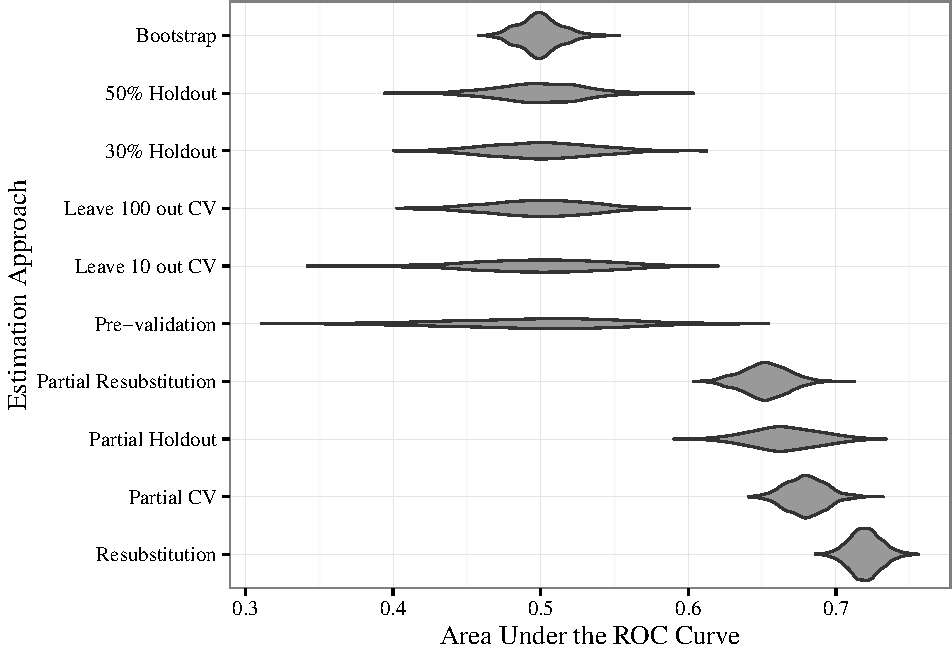
\includegraphics{paper-revised_files/figure-latex/cvsims-1.pdf}
\caption{Comparison of different approaches to estimating the Area Under
the ROC Curve (AUC) in the setting where a dataset is used to both
develop the signature and evaluate its performance. The violin plots
show mirrored density estimates for the AUC for 1000 replicates of the
numerical experiment. In each replicate, there are 1000 observations and
500 features. The true value of the AUC is 0.5. CV = Cross validation.
\label{fig1}}
\end{figure}

\begin{figure}[htbp]
\centering
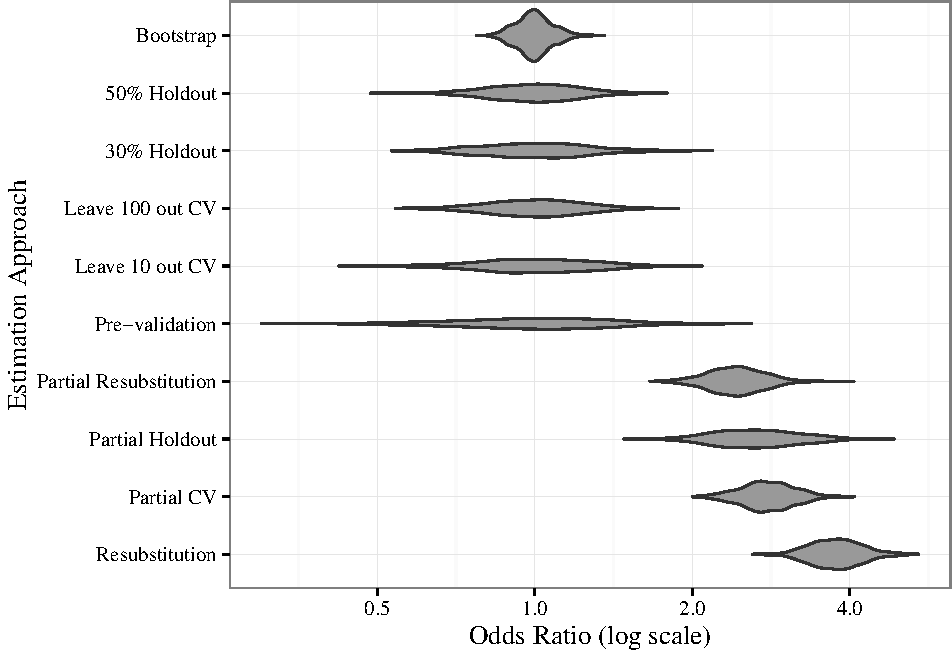
\includegraphics{paper-revised_files/figure-latex/cvsims2-1.pdf}
\caption{Comparison of different approaches to estimating the odds ratio
(OR) in the setting where a dataset is used to both develop the
signature and evaluate its performance. The violin plots show mirrored
density estimates for the log OR for 1000 replicates of the numerical
experiment. In each replicate, there are 1000 observations and 500
features. The true value of the OR is 1.0. CV = Cross validation.
\label{fig2}}
\end{figure}

\begin{longtable}[c]{@{}lrrrrrr@{}}
\caption{Comparison of different approaches to estimating the Area Under
the ROC Curve (AUC) and the log odds ratio (OR) in the setting where a
dataset is used to both develop the signature and evaluate its
performance. The true value of the AUC is 0.5 and the true value of the
Log OR is 0.0. Estimates are based on 1000 replicates of the numerical
experiment. In each replicate, there are 1000 observations and 500
features. CV = Cross validation.}\tabularnewline
\toprule
Approach & mean AUC & std.dev AUC & Bias AUC & mean OR & std.dev OR &
Bias OR\tabularnewline
\midrule
\endfirsthead
\toprule
Approach & mean AUC & std.dev AUC & Bias AUC & mean OR & std.dev OR &
Bias OR\tabularnewline
\midrule
\endhead
Resubstitution & 0.72 & 0.01 & 0.22 & 1.33 & 0.12 & 1.33\tabularnewline
Partial CV & 0.68 & 0.01 & 0.18 & 1.02 & 0.12 & 1.02\tabularnewline
Partial Holdout & 0.67 & 0.02 & 0.17 & 0.97 & 0.19 & 0.97\tabularnewline
Partial Resubstitution & 0.65 & 0.02 & 0.15 & 0.88 & 0.12 &
0.88\tabularnewline
Pre-validation & 0.50 & 0.05 & 0.00 & -0.01 & 0.32 &
-0.01\tabularnewline
Leave 10 out CV & 0.50 & 0.04 & 0.00 & 0.00 & 0.25 & 0.00\tabularnewline
Leave 100 out CV & 0.50 & 0.03 & 0.00 & 0.00 & 0.20 &
0.00\tabularnewline
30\% Holdout & 0.50 & 0.03 & 0.00 & 0.00 & 0.24 & 0.00\tabularnewline
50\% Holdout & 0.50 & 0.03 & 0.00 & 0.00 & 0.20 & 0.00\tabularnewline
Bootstrap & 0.50 & 0.01 & 0.00 & 0.00 & 0.08 & 0.00\tabularnewline
\bottomrule
\end{longtable}

Not surprisingly, the resubstitution estimates are optimistically
biased: the naive resubstitution estimate of the AUC is 44\% larger than
it should be and the log OR estimate is over 2 times higher than it
should be, on average. Partial resubstitution, partial holdout, and
partial cross-validation estimates do not ameliorate the bias very much.
Investigators are tempted to use partial holdout estimates as it is more
convenient to not have to carry along a large number of feature
measurements into the modeling part of the signature development
process, and they may think that the resulting performance estimates are
still close to valid, as only half of the data are used to form the
estimates. However, here we see that these versions are still severely
biased and should not be reported as valid assessments of the
performance of biomarker signatures.

The split-sample holdout, cross-validation, bootstrap, and
pre-validation methods all produce esentially unbiased estimates in the
simulated example, with their mean AUCs being nearly 0.5 and the mean
ORs being nearly 1. We can compare the spread of the distributions to
get a sense of the differences in precision of the estimates. The
bootstrap approach appears to be the most precise, followed by the
cross-validation, holdout, and finally the pre-validation. The
bootstrap, as intended, is a more efficient, smoothed version of the
cross validation estimate (Figure \ref{fig1}, \ref{fig2}). It provides
the best balance between allocating data to train the signature and
having independent data remaining to precisely estimate the statistic
\(\phi\).

\subsection{Data Analysis}\label{data-analysis}

\subsection{Data analysis example}\label{data-analysis-example}

We now illustrate the concepts and methods just discussed by reanalyzing
data that had been used to build a previously published lung cancer
prognostic signature \citet{zhu2010prognostic}. Briefly, the data of
interest are from the JBR.10 trial, which was a randomized controlled
trial of the adjuvant chemotherapy regimen vinorelbine/cisplatin (ACT)
versus observation alone (OBS) in 482 participants with non small cell
lung cancer (NSCLC) who had undergone surgery. Of those 482
participants, 169 had frozen tumor tissue collected, and of those tumor
samples, 133 (71 in ACT and 62 in OBS) had gene-expression profiling
performed using U133A oligonucleotide microarrays (Affymetrix, Santa
Clara, CA).

The goal of the \citet{zhu2010prognostic} paper was to identify a
multi-gene signature that strongly predicts prognosis, and the
hypothesis was that the poor prognosis subgroup would benefit more from
ACT than the good prognosis subgroup. The signature was developed on a
training data set (``trained'') to predict disease specific survival.
The annotated gene expression data and clinical information are
available from the Gene Expression Omnibus database(identifier:
GSE14814, \citet{edgar2002gene}).

\citet{zhu2010prognostic} present results that mainly focus on the
association of their signature with outcome, albeit a less than ideal
measure of discrimination ability. They demonstrate that the two risk
subgroups predicted by their signature (high risk and low risk) have
separation in their survival curves and that the hazard ratio for their
signature is large and significant even when adjusting for other risk
factors. They do not directly address calibration, that is, whether
their signature accurately predicts survival times.

We used a similar approach to preprocessing as did
\citet{zhu2010prognostic}, although we could not reproduce their
workflow exactly due to outdated software. Batch effects were removed
using the \texttt{ComBat} function in the \texttt{sva} \texttt{R}
package \citep{leeksva} and then the gene expression values were
centered by their means and scaled by their standard deviations. Our
signature development approach is similar but not identical to that in
\citet{zhu2010prognostic}. For purposes of illustrating the concepts we
used a simplified approach to signature development that retains the
main characteristics of the original method. The exact approach to
signature development does not have a major impact on the main
conclusions of our evaluation of the various approaches to signature
performance assessment.

After processing the data as described above, we performed a gene
selection step wherein we fit univariate Cox regression models with
disease specific survival as the outcome and each gene as the single
predictor. Genes with univariate p-values less than 0.005 were
preliminarily selected for further analysis. Then, each gene from the
preliminary list was weighted by its univariate Cox regression
coefficient, and the resulting weighted gene expression values were
summed to form risk scores. Genes were selected for inclusion in the
risk score in a forward selection manner. Starting with the most
significant weighted gene, the gene that when added to the risk score
improved the concordance between survival times and the risk score most
was selected next. If no gene improved the concordance, the process was
stopped. All genes on the final selected list were included in a
multivariable Cox regression model to fit the final risk score with new
coefficients. We selected the cutoff that split the patients into two
risk groups corresponding to the smallest log-rank statistic p-value
when applied to the continuous risk score.

The signature development procedure was described in the introduction.
There is both a feature selection step, and a multivariable estimation
step. This results in a continuous signature which is the linear
predictor of a Cox regression model. The signature is dichotomized by
selecting the cutoff that yields the most significant log-rank statistic
for comparing the resulting risk groups. Discrimination of the signature
is assessed using the concordance statistic as implemented in the
\texttt{survival} package in \texttt{R} \citep{survival}. To paraphrase
the help file: this is defined as the probability of agreement for any
two randomly chosen observations, which in this case means that the
observation with the shorter survival time also has the larger signature
value. This is similar to an interpretation of the AUC for binary data.

First we fit the signature using the entire observation cohort (n = 62).
The signature was then evaluated on the same dataset. The survival plot
on the left side of Figure \ref{fig2} shows extreme separation between
the two risk groups (HR = 20, p \textless{} 0.001), consistent with the
reported JBL.10 signature, and the estimated concordance is 0.87. After
correctly accounting for the selection process, our estimates of
association and discrimination are much less impressive.

The right plot in Figure \ref{fig2} shows the survival curves for the
two risk groups using the pre-validated estimates of the risk score. We
partitioned the 62 observations into 8 groups of 6 and 2 groups of 7.
Then for each group \(b\), we fit the model using \(S_{-b}\) and
obtained prevalidated estimates for \(S_{b}\). The survival curves plot
the survival times for comparing risk groups using the prevalidated
estimates. The separation is much less impressive. The concordance
between the prevalidated signature and the survival times is 0.61,
indicating much worse discrimination.

\begin{figure}[htbp]
\centering
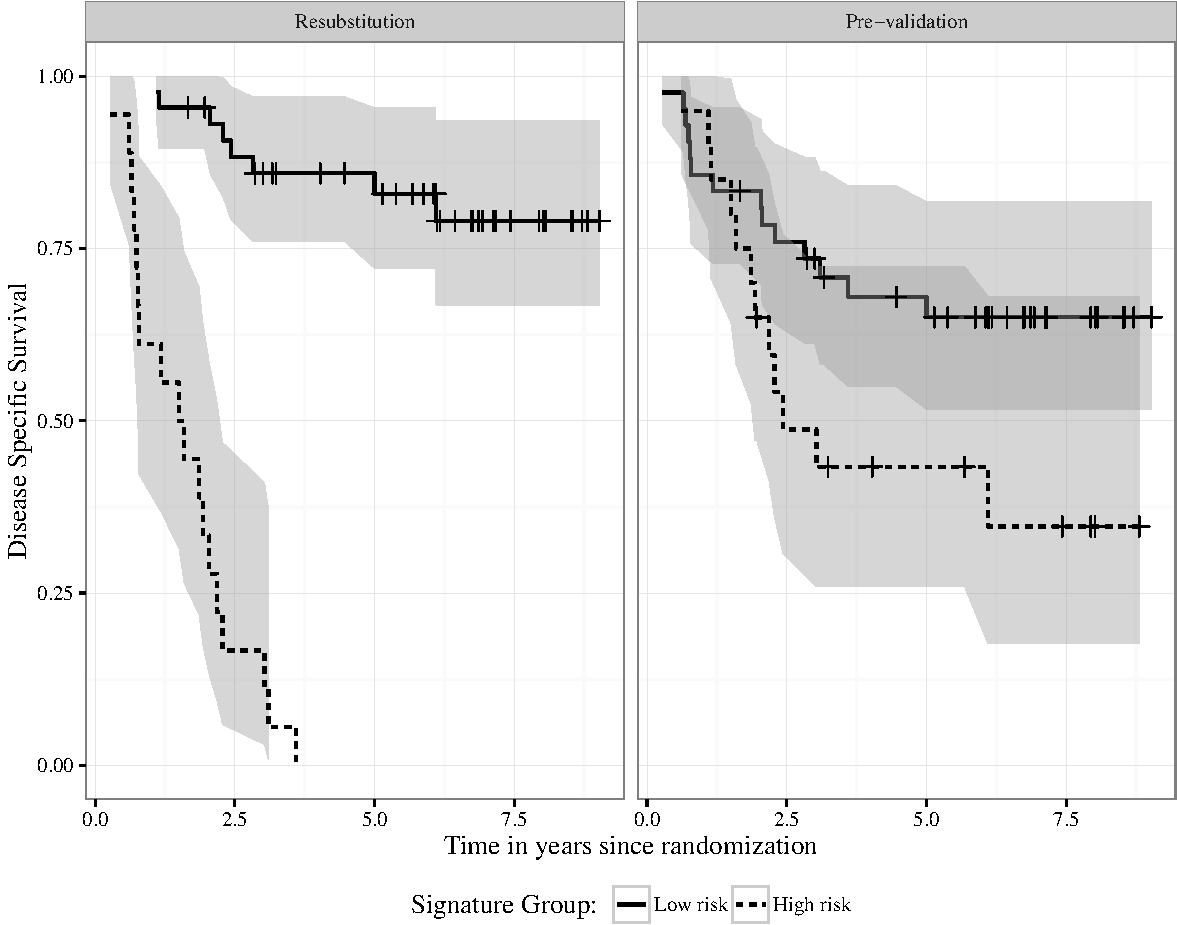
\includegraphics{paper-revised_files/figure-latex/examppresub-1.pdf}
\caption{Comparison of survival by gene expression based risk signature.
The left plot shows the resubstitution estimate, while the right plot
shows the pre-validated estimate. \label{fig2}}
\end{figure}

\begin{figure}[htbp]
\centering
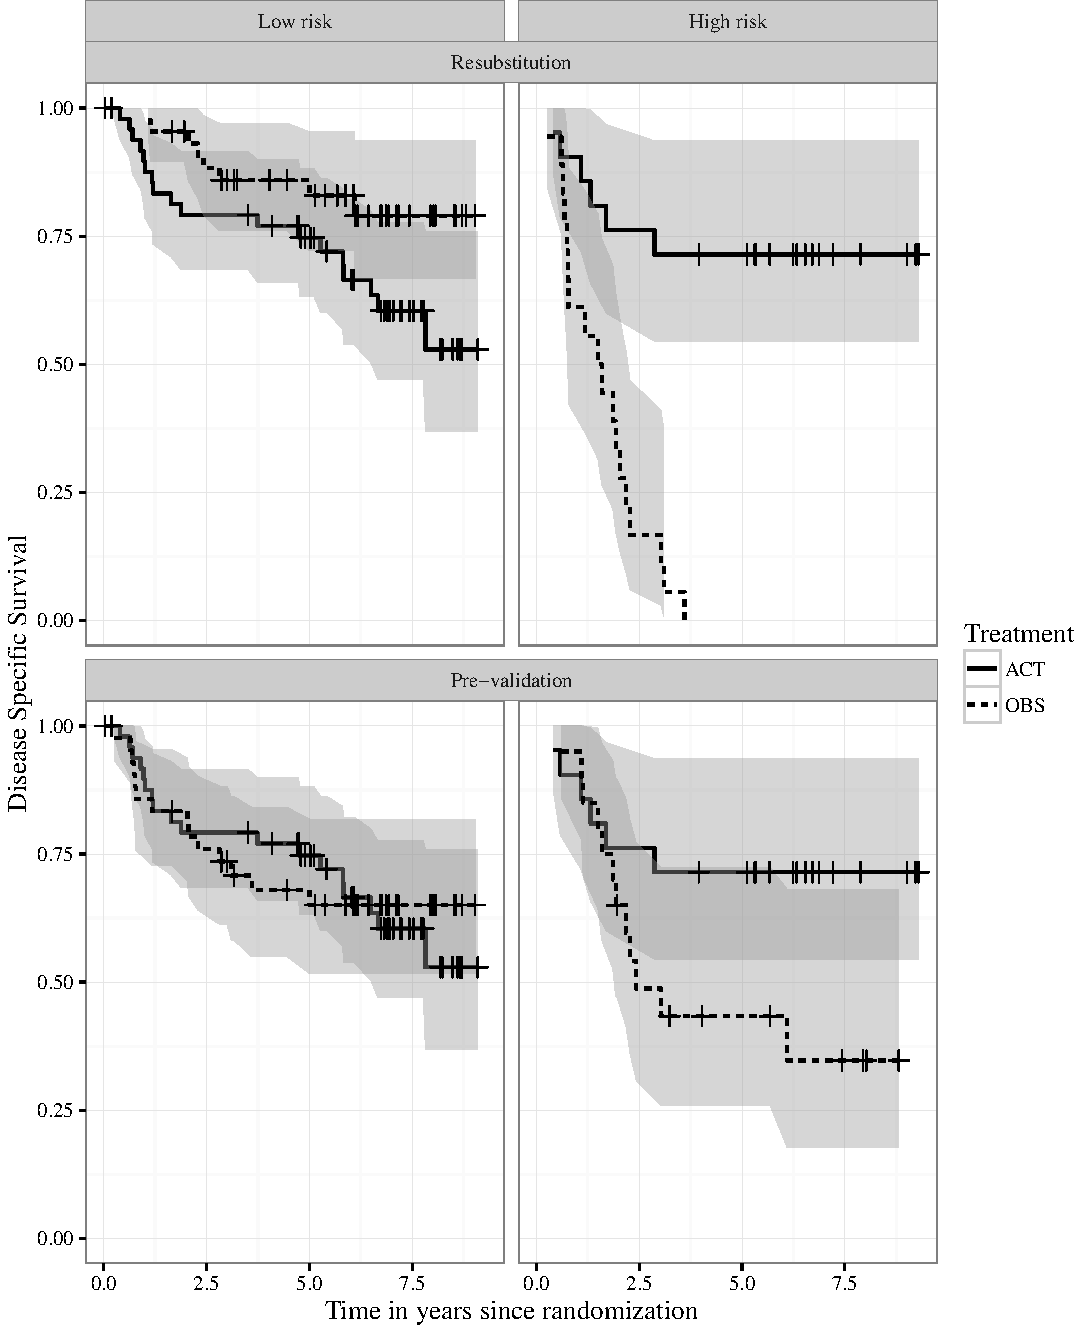
\includegraphics{paper-revised_files/figure-latex/inter1-1.pdf}
\caption{Survival curves comparing the treatment effect by gene
expression signature risk group. The top set of plots shows the partial
resubstitution based signature and the bottom row shows the
pre-validated signature estimates. \label{fig3}}
\end{figure}

\begin{longtable}[c]{@{}lllll@{}}
\caption{Hazard ratios and 95\% confidence intervals from separate Cox
regression models that adjust for tumor histologic subtype, stages, age,
and sex. Rows labeled `High risk vs low risk' show the hazard ratio for
the signature-based risk group comparison. The rows labeled `Trt/Risk
interaction' show the hazard ratio for the interaction term of treatment
by signature-based risk group. The partial substitution estimates are
dramatically optimistically biased. \label{adjhr}}\tabularnewline
\toprule
Method & Comparison & Hazard Ratio & 95\% CI & Adjusted p\tabularnewline
\midrule
\endfirsthead
\toprule
Method & Comparison & Hazard Ratio & 95\% CI & Adjusted p\tabularnewline
\midrule
\endhead
\textbf{Partial Resubstitution} & High Risk vs Low Risk & 38.9 & 9.2 to
164.7 & \textless{} 0.001\tabularnewline
& Trt/Risk interaction & 14.7 & 3.2 to 67.0 & \textless{}
0.001\tabularnewline
\textbf{Prevalidation} & High Risk vs Low Risk & 1.9 & 0.8 to 4.3 &
0.122\tabularnewline
& Trt/Risk interaction & 1.8 & 0.5 to 6.5 & 0.395\tabularnewline
\bottomrule
\end{longtable}

We also show plots to assess the ability of the signature to be useful
for treatment selection (Figure \ref{fig3}). These plots show the
survival curves comparing treatment arms grouped in panels by the risk
score. As described by \citet{polley2013statistical}, the idea is to
determine whether the treatment is beneficial in one group and not
benficial or harmful in another group, indicating that different
treatment decisions would be made based on the signature. On one hand,
the overfit signature shows dramatic differences in treatment efficacy
between the low risk and high risk groups. In fact it appears that the
treatment is harmful in the low risk group, but highly beneficial in the
high risk group. The prevalidated signature on the other hand, shows
differences that are much less dramatic. It appears that the treatment
is mildly beneficial in both groups, possibly to a higher degree in the
high risk group. This suggests that the dramatic predictive value of the
signature was merely an artifact of overfitting the signature to the OBS
arm data. \citet{simon2011re} explain the flaws in this type of approach
in which one attempts to develop a signature for treatment selection by
developing a prognostic signature on data from the control arm of a
trial and then applying that signature to both the control and
experimental arm data to establish predictiveness.

In a multivariable Cox model we observe similar trends when comparing
the prevalidated signature to the overfit signature. We fit two
regression models. In the first, the aim is to assess the prognostic
value of the signature by estimating the hazard ratio for the high risk
versus low risk groups, adjusted for tumor histologic subtype, stage,
age, and sex. In the second model, the idea is to assess the predictive
value of the signature by estimating the treatment by signature
interaction effect, adjusting for the same clinical covariates. The
results are reported in Table \ref{adjhr}. The full model summaries are
report in Table \ref{multimodel}. For the partial resubstitution
approach, we find an extreme hazard ratio of nearly 40 for the
prognostic effect, and a strong and significant treatment by signature
interaction. Using the prevalidated signature, the effect estimates are
much smaller and of small magnitude in comparison to the standard
clinical features. Note that the inference from the pre-validated model
is not exactly correct either, because the resampling procedure induces
a correlation among the observations (the prevalidated signature values
are estimated from heavily overlapping data). Despite this, these
results are unimpressive and would not be considered promising for
clinical use.

\citet{zhu2010prognostic} should be commended for their commitment to
making their data, methods, and analysis code publically available,
which allowed us to reanalyze their study data. More often, methods used
to derive signatures are vaguely and incompletely presented and a
resubstitution analysis or other flawed approach goes undetected or can
be discovered only through a very careful scrutiny of the methods and
supplementary materials.

\begin{table}[!htbp] \centering 
  \caption{Complete Results of Multivariable Regression Models. Entries are hazard ratios and 95 percent confidence intervals.  \label{multimodel}} 
  \label{} 
\begin{tabular}{@{\extracolsep{5pt}}lcccc} 
\\[-1.8ex]\hline 
\hline \\[-1.8ex] 
 & \multicolumn{4}{c}{\textit{Dependent variable:}} \\ 
\cline{2-5} 
\\[-1.8ex] & \multicolumn{4}{c}{Disease-specific Survival} \\ 
 & Resubstitution & Prevalidation & Resubstitution & Prevalidation \\ 
\\[-1.8ex] & (1) & (2) & (3) & (4)\\ 
\hline \\[-1.8ex] 
 High Risk & 38.9$^{***}$ & 1.9 & 0.7 & 1.0 \\ 
  & (9.2 to 164.7) & (0.8 to 4.3) & (0.3 to 2.0) & (0.4 to 2.7) \\ 
  & & & & \\ 
 Trt: OBS &  &  & 0.5 & 1.3 \\ 
  &  &  & (0.2 to 1.3) & (0.6 to 2.8) \\ 
  & & & & \\ 
 Male Gender & 1.3 & 1.4 & 1.2 & 1.4 \\ 
  & (0.4 to 3.8) & (0.5 to 4.2) & (0.6 to 2.4) & (0.7 to 2.8) \\ 
  & & & & \\ 
 Stage > I & 2.1$^{*}$ & 2.7$^{**}$ & 2.0$^{**}$ & 2.3$^{***}$ \\ 
  & (0.9 to 4.7) & (1.2 to 6.3) & (1.1 to 3.6) & (1.3 to 4.1) \\ 
  & & & & \\ 
 Age in Years & 1.0 & 1.1$^{**}$ & 1.0$^{*}$ & 1.1$^{***}$ \\ 
  & (0.9 to 1.1) & (1.0 to 1.1) & (1.0 to 1.1) & (1.0 to 1.1) \\ 
  & & & & \\ 
 Histology: LCUC & 1.7 & 2.7 & 1.5 & 1.9 \\ 
  & (0.5 to 6.3) & (0.8 to 10.0) & (0.6 to 3.7) & (0.7 to 4.7) \\ 
  & & & & \\ 
 Histology: SQCC & 3.4$^{*}$ & 0.4$^{**}$ & 0.8 & 0.4$^{***}$ \\ 
  & (0.9 to 13.3) & (0.2 to 1.0) & (0.3 to 1.7) & (0.2 to 0.8) \\ 
  & & & & \\ 
 High Risk * Trt:OBS &  &  & 14.7$^{***}$ & 1.8 \\ 
  &  &  & (3.2 to 67.0) & (0.5 to 6.5) \\ 
  & & & & \\ 
\hline \\[-1.8ex] 
Observations & 62 & 62 & 133 & 133 \\ 
Score (Logrank) Test & 69.6$^{***}$ (df = 6) & 21.5$^{***}$ (df = 6) & 84.5$^{***}$ (df = 8) & 32.0$^{***}$ (df = 8) \\ 
\hline 
\hline \\[-1.8ex] 
\textit{Note:}  & \multicolumn{4}{r}{$^{*}$p$<$0.1; $^{**}$p$<$0.05; $^{***}$p$<$0.01} \\ 
\end{tabular} 
\end{table}

\section{Discussion}\label{discussion}

Examples of flawed approaches such as naive resubstitution, partial
resubstitution, partial holdout, and partial CV remain very common in
the published literature more than a decade after many high-dimensional
molecular assays were first introduced. All performance metrics, whether
they assess calibration or discrimination or something else, are subject
to bias in estimation due to overfitting. Strategies to avoid this type
of bias are well-studied in the statistical literature and here we have
demonstrated how they can be implemented in a real clinical example. The
ability to perform the kind of in-depth data reanalysis we performed on
the example in this paper is usually limited by restrictions on data
access and insufficient description of analysis methods. Sadly, reports
of strong associations with overfit biomarker signatures are all too
common in the medical literature. The amount of bias that is possible is
not known and can be difficult to decipher based on study reports. It is
imperative that investigators and journal editors take overfitting bias
seriously to ensure that signature performance claims are valid.
Unfortunately this often results in study reports that are far less
optimistic than usual.

The \citet{zhu2010prognostic} paper used the approach of identifying a
signature using the control arm of the trial, evaluating it using the
combined control and treatment arms, and then hoping that the signature
would be useful for treatment selection. This approach has been shown to
be invalid \citep{simon2011re} for identifying a predictive signature,
and indeed we show that the resubstitution aspect of the evaluation
likely led to overstatments of the size of the signature effect.
Properly doing cross-validation for estimating the calibration of the
signature and doing pre-validation for assessment of the discrimination
of the signature show that the associations are much more modest.

When we assess the signature on the independent treatment arm, we see
that there is no significant difference between the risk groups. This
raises the question of whether it is appropriate to use non-random
splits of the dataset in order to obtain valid estimates of the
calibration or discrimination. Instead of treatment arms, we could
imagine a large multi-center study, and we could split the data into
disjoint subgroups based on the center. Specifically, suppose we split
the development dataset \(S\) into \(S_1\) and \(S_2\) according to a
discrete covariate \(X\) that takes on levels 1 or 2. The we develop a
signature \(f_{S_1}\) using \(S_1\) and evaluate it on \(S_2\) by
estimating \(\hat{E}[\phi_{f_{S_1}}(S_2)]\). This is an estimate not of
\(E_\mathcal{P}[\phi_f(S)]\), but rather
\(E_{\mathcal{P}_2}[\phi_f(S)]\), where \(\mathcal{P}_2\) is the
distribution for the sub-population with \(X = 2\) that \(S_2\) is a
sample from. This estimate would only be recommended if the signature is
intended for use in that specific subpopulation, and if that were the
case, then it doesn't make much sense to develop the signature using the
subpopulation \(\mathcal{P}_1\). If these groups differed substantially,
then we would not expect the signature to perform adequately. The
differences in performance may depend on many factors, including how
\(X\) is associated with the distribution of the features and the
outcome. If a signature becomes broadly used in clinics, these
center-to-center differences would be important to assess as a part of
signature efficacy surveillance.

\section{Note}\label{note}

All analysis code and the source files for this manuscript are available
from the authors' webpage.

\renewcommand\refname{References}
\bibliography{paper}

\end{document}
